\begin{enumerate}
    \item Calculate the conditional probabilities given by the figure.\\
    Precalculation:
    \begin{align*}
        P(A)&=0.01+0.02+0.05+0.04+0.08+0.05+0.07=0.32\\
        P(B)&=0.08+0.06+0.13+0.11+0.05+0.02+0.01=0.46\\
        P(C)&=0.11+0.07+0.04+0.08+0.02+0.05+0.11=0.48
    \end{align*}
    Calculate:
    \begin{enumerate}
        \item $\displaystyle P(A|B)=\frac{P(A\cap B)}{P(B)}=\frac{0.01+0.02+0.05}{0.46}=4/23$
        \item $\displaystyle P(C|A)=\frac{P(A\cap C)}{P(A)}=\frac{0.02+0.05+0.04+0.08}{0.32}=19/32$
        \item $\displaystyle P(B|A\cap B)=\frac{P(A\cap B \cap B)}{P(A\cap B)} = 1$
        \item $\displaystyle P(B|A\cup B)=\frac{P(B)}{P(A\cup B)}=\frac{0.46}{P(A)+0.08+0.06+0.13+0.11}=0.46/0.7=23/35$
        \item $\displaystyle P(A|A\cup B\cup C)=\frac{P(A)}{P(A\cup B\cup C)}=\frac{0.32}{1-0.04-0.05-0.03}=4/11$
        \item $\displaystyle P(A\cap B|A\cup B)=\frac{P(A\cap B)}{P(A\cup B)}=\frac{0.01+0.02+0.05}{0.7}=0.08/0.7=4/35$
    \end{enumerate}

    \item When a company receives an order, there is a probability of 0.42 that its value is over \$1000. If an order is valued at over \$1000, then there is a probability of 0.63 that the customer will pay with a credit card.\\
    \begin{enumerate}
        \item What is the probability that the next 3 independent orders will each be valued at over \$1000?
        $$P((>\$1000)\times 3)=P(>\$1000)^3=0.42^3=0.074088$$
        \item What is the probability that the next order will be valued at over \$1000 but will not be paid with a credit card?
        $$P(\n{card}|>\$1000)=1 - P(\n{not card}|>\$1000)= 1-0.63 = 0.37$$
        $$P(>\$1000\cap\n{card})=P(>\$1000)\times P(\n{card}|>\$1000)=0.42\times0.37=0.1554$$
    \end{enumerate}

    \item A card is drawn at random from a pack of cards. Calculate:
    \begin{enumerate}
        \item $P(\n{A}\heartsuit|\n{card from red suit})=1/26$
        \item $P(\n{heart}|\n{card from red suit})=13/26=0.5$
        \item $P(\n{card from black suit})=26/52=0.5$
        \item $P(\n{heart}|\n{card from black suit})=0$
        \item $P(\n{king}|\n{card from red suit})=2/26=1/13$
        \item $P(\n{king}|\n{red picture card})=2/6=1/3$
    \end{enumerate}
    \item A ball is chosen at random from a bag containing 150 balls that are either red or blue and either dull or shiny. There are 36 red shiny balls and 54 blue balls. What is the probability of the chosen ball being shiny conditional on it being red? What is the probability of the chosen ball being dull conditional on it being red?
    \begin{align*}
        |\n{red}|&=150-|\n{blue}|=150-54=96\\
        |\n{red}\cap \n{dull}|&=|\n{red}|-|\n{red}\cap\n{shiny}|=96-36=60\\
        P(\n{shiny}|\n{red})&=|\n{red}\cap\n{shiny}|/|red|=36/96=3/8\\
        P(\n{red}\cap\n{dull}|\n{red})&=60/96=5/8
    \end{align*}

    \item A manufactured component has its quality graded on its performance, appearance and cost. Each of these 3 characteristics is graded as either pass or fail. There is a probability of 0.4 that a component passes on both appearance and cost. There is a probability of 0.31 that a component passes on all 3 characteristics. There is a probability of 0.64 that a component passes on performance. There is a probability of 0.19 that a component fails on all 3 characteristics. There is a probability of 0.06 that a component passes on appearance but fails on both performance and cost.
    % Edit from https://www.overleaf.com/latex/templates/homework-template-coding-theory-course/rhrshkpjnhpb
    \begin{center}
        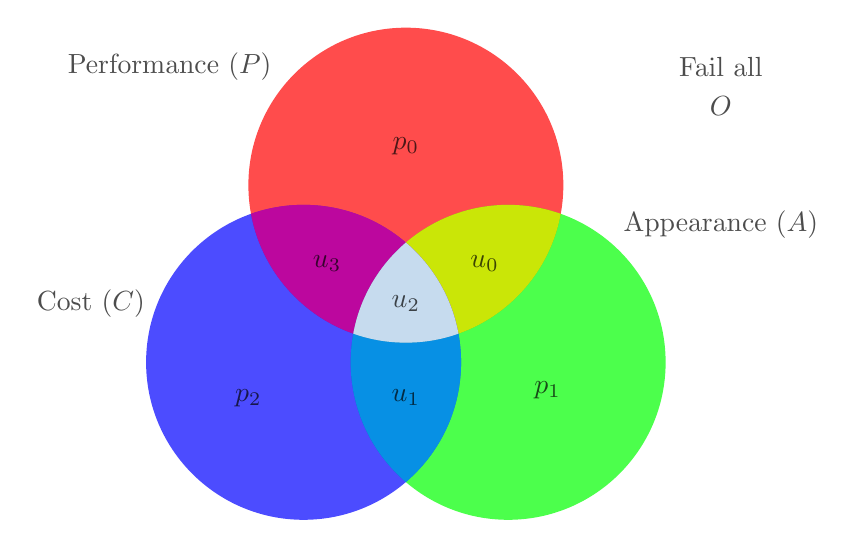
\begin{tikzpicture}[thin,fill opacity=0.7]
        \draw [draw=none, fill=red] (90:1.5) circle (2cm);
        \draw [draw=none, fill=green] (-30:1.5) circle (2cm);
        \draw [draw=none, fill=blue] (210:1.5) circle (2cm);
        \begin{scope}
            \clip (90:1.5) circle(2cm);
            \draw [draw=none, fill=yellow] (-30:1.5) circle (2cm);
        \end{scope}
        \begin{scope}
            \clip (210:1.5) circle(2cm);
            \draw [draw=none, fill=magenta] (90:1.5) circle (2cm);
        \end{scope}
        \node at (-3,3) {Performance ($P$)};
        \node at (-4,0) {Cost ($C$)};
        \node at (4,1) {Appearance ($A$)};
        \node at (4,3) {Fail all};
        \begin{scope}
            \clip (-30:1.5) circle(2cm);
            \draw [draw=none, fill=cyan] (210:1.5) circle (2cm);
        \end{scope}
        \begin{scope}
            \clip (90:1.5) circle(2cm);
            \clip (210:1.5) circle(2cm);
            \draw [draw=none, fill=white] (-30:1.5) circle (2cm);	
        \end{scope}
        \node at (1,.5) {$u_0$};
        \node at (0,0) {$u_2$};
        \node at (1.8,-1.1) {$p_1$};
        \node at (-1,.5) {$u_3$};
        \node at (0,-1.2) {$u_1$};
        \node at (0,2) {$p_0$};
        \node at (-2,-1.2) {$p_2$};
        \node at (4,2.5) {$O$};
        \end{tikzpicture}
    \end{center}
    Using a Venn diagram to summarize the problem:
    \begin{align*}
        u_1 + u_2&= 0.4 & u_2&= 0.31 & p_1 &= 0.06\\
        p_0 + u_3 + u_2 + u_0&= 0.64 & O&= 0.19\\
    \end{align*}
    Hence: $u_1 = 0.4-0.31=0.09$
    \begin{enumerate}
        \item What is the probability that a component passes on cost but fails on both performance and appearance?
        $$P(C\backslash P\backslash A)=p_2=1-u_1-p_1-O-(p_0+u_3+u_2 +u_0)=1-0.09-0.06-0.19-0.64=0.02$$
        \item If a component passes on both appearance and cost, what is the probability that it passes on all 3 characteristics?
        $$P(APC|AC)=\frac{P(APC)}{P(AC)}=\frac{u_2}{u_2+u_1}=0.31/0.4=31/40=0.775$$
    \end{enumerate}
\end{enumerate}